%%%%%%%%%%%%%%%%%%%%%%%%%%%%%%%%%%%%%%%%%
% Beamer Presentation
% LaTeX Template
% Version 1.0 (10/11/12)
%
% This template has been downloaded from:
% http://www.LaTeXTemplates.com
%
% License:
% CC BY-NC-SA 3.0 (http://creativecommons.org/licenses/by-nc-sa/3.0/)
%
%%%%%%%%%%%%%%%%%%%%%%%%%%%%%%%%%%%%%%%%%

%----------------------------------------------------------------------------------------
%	PACKAGES AND THEMES
%----------------------------------------------------------------------------------------

\documentclass[handout]{beamer}

\mode<presentation> {

% The Beamer class comes with a number of default slide themes
% which change the colors and layouts of slides. Below this is a list
% of all the themes, uncomment each in turn to see what they look like.

%\usetheme{default}
%\usetheme{AnnArbor}
%\usetheme{Antibes}
%\usetheme{Bergen}
%\usetheme{Berkeley}
%\usetheme{Berlin}
%\usetheme{Boadilla}
%\usetheme{CambridgeUS}
%\usetheme{Copenhagen}
%\usetheme{Darmstadt}
%\usetheme{Dresden}
%\usetheme{Frankfurt}
%\usetheme{Goettingen}
%\usetheme{Hannover}
%\usetheme{Ilmenau}
%\usetheme{JuanLesPins}
%\usetheme{Luebeck}
\usetheme{Madrid}
%\usetheme{Malmoe}
%\usetheme{Marburg}
%\usetheme{Montpellier}
%\usetheme{PaloAlto}
%\usetheme{Pittsburgh}
%\usetheme{Rochester}
%\usetheme{Singapore}
%\usetheme{Szeged}
%\usetheme{Warsaw}

% As well as themes, the Beamer class has a number of color themes
% for any slide theme. Uncomment each of these in turn to see how it
% changes the colors of your current slide theme.

%\usecolortheme{albatross}
%\usecolortheme{beaver}
%\usecolortheme{beetle}
%\usecolortheme{crane}
%\usecolortheme{dolphin}
%\usecolortheme{dove}
%\usecolortheme{fly}
%\usecolortheme{lily}
%\usecolortheme{orchid}
%\usecolortheme{rose}
%\usecolortheme{seagull}
%\usecolortheme{seahorse}
%\usecolortheme{whale}
%\usecolortheme{wolverine}

%\setbeamertemplate{footline} % To remove the footer line in all slides uncomment this line
%\setbeamertemplate{footline}[page number] % To replace the footer line in all slides with a simple slide count uncomment this line

%\setbeamertemplate{navigation symbols}{} % To remove the navigation symbols from the bottom of all slides uncomment this line
}

\usepackage{graphicx} % Allows including images
\usepackage{booktabs} % Allows the use of \toprule, \midrule and \bottomrule in tables
\usepackage{cool}
\usepackage{tikz}
\usepackage{amsmath}
\usepackage{pseudocode}
\usepackage{MnSymbol,wasysym}
\DeclareMathOperator*{\argmax}{argmax}
\DeclareMathOperator*{\argmin}{argmin}
\usetikzlibrary{positioning}

%----------------------------------------------------------------------------------------
%	TITLE PAGE
%----------------------------------------------------------------------------------------

\title[Optimal Market-Making]{Stochastic Control for Optimal Market-Making} % The short title appears at the bottom of every slide, the full title is only on the title page

\author{Ashwin Rao} % Your name
\institute[Stanford] % Your institution as it will appear on the bottom of every slide, may be shorthand to save space
{
ICME, Stanford University
 % Your institution for the title page
}

\date{\today} % Date, can be changed to a custom date

\begin{document}
\begin{frame}
\titlepage % Print the title page as the first slide
\end{frame}

\begin{frame}
\frametitle{Overview} % Table of contents slide, comment this block out to remove it
\tableofcontents % Throughout your presentation, if you choose to use \section{} and \subsection{} commands, these will automatically be printed on this slide as an overview of your presentation
\end{frame}

\section{Trading Order Book Dynamics}

\begin{frame}
\frametitle{Trading Order Book (TOB)}
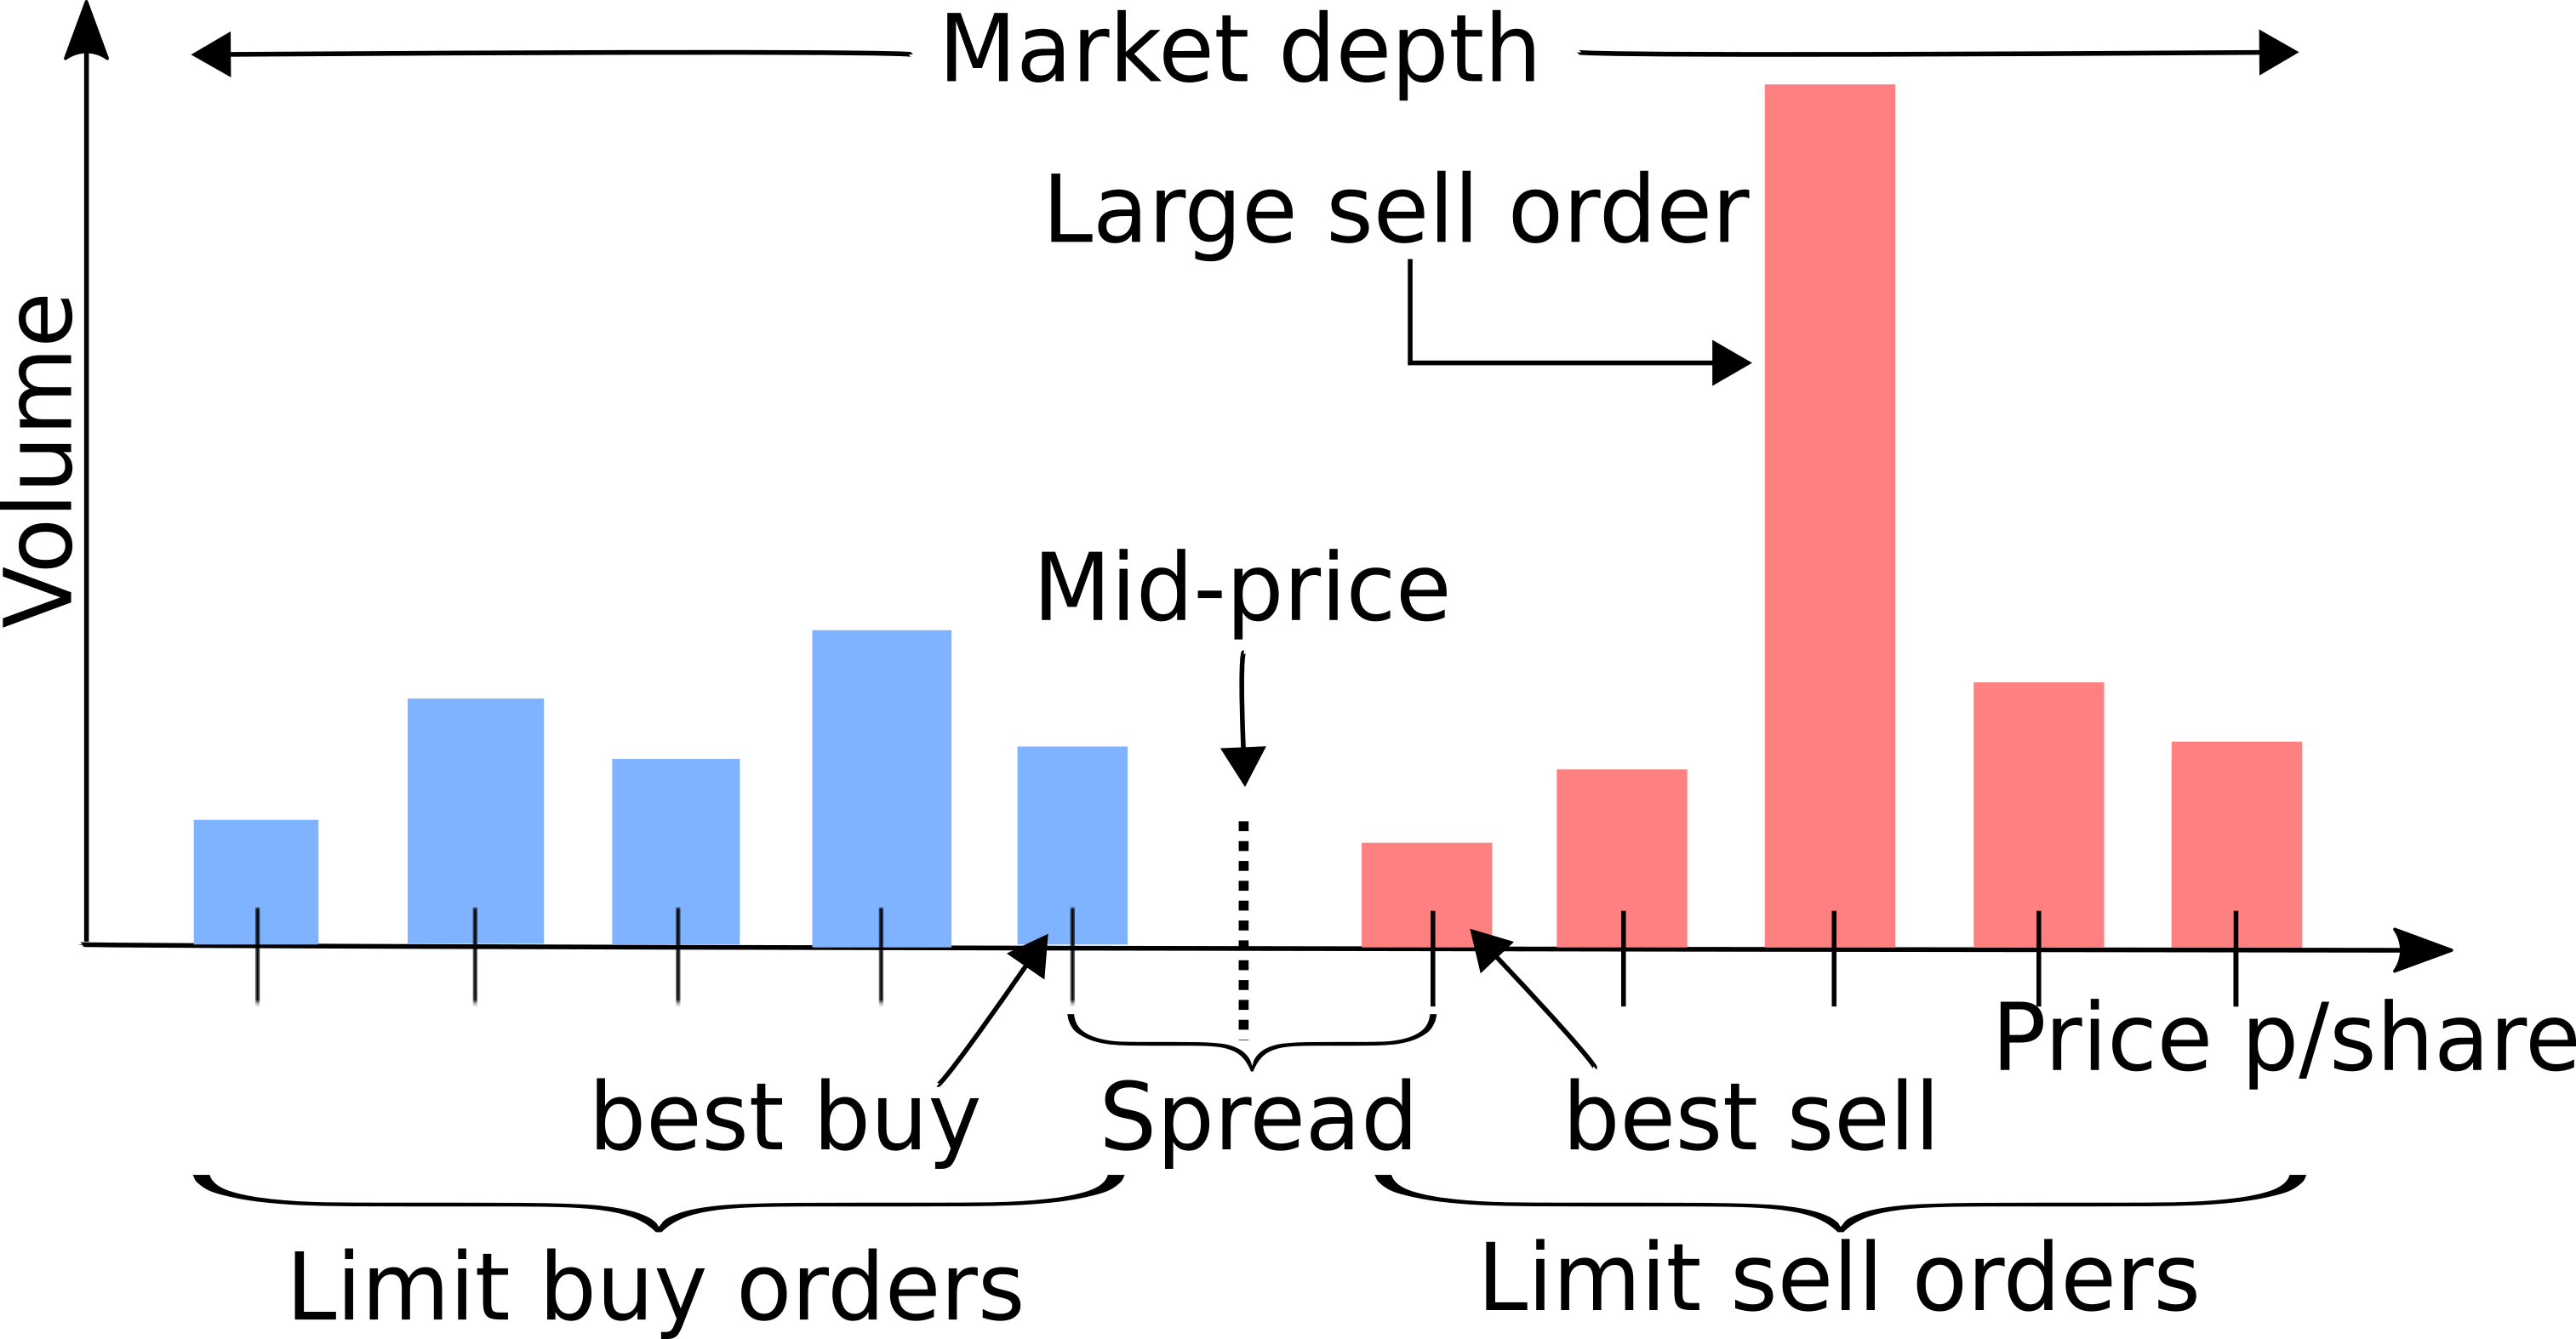
\includegraphics[width=11.5cm, height=7cm]{order_book.png}
\end{frame}

\begin{frame}
\frametitle{Basics of Trading Order Book (TOB)}
\pause
\begin{itemize}[<+->]
\item Buyers/Sellers express their intent to trade by submitting bids/asks
\item These are Limit Orders (LO) with a price $P$ and size $N$
\item Buy LO $(P, N)$ states willingness to buy $N$ shares at a price $\leq P$
\item Sell  LO $(P, N)$ states willingness to sell $N$ shares at a price $\geq P$
\item Trading Order Book aggregates order sizes for each unique price
\item So we can represent with two sorted lists of (Price, Size) pairs
$$\mbox{Bids: } [(P_i^{(b)}, N_i^{(b)}) \mid 1 \leq i \leq m], P_i^{(b)} > P_j^{(b)} \mbox{ for } i < j$$
$$\mbox{Asks: } [(P_i^{(a)}, N_i^{(a)}) \mid 1 \leq i \leq n], P_i^{(a)} < P_j^{(a)} \mbox{ for } i < j$$
\item We call $P_1^{(b)}$ as simply {\em Bid}, $P_1^{(a)}$ as {\em Ask}, $\frac {P_1^{(a)} + P_1^{(b)}} 2$ as {\em Mid}
\item We call $P_1^{(a)} - P_1^{(b)}$ as {\em Spread}, $P_n^{(a)} - P_m^{(b)}$ as {\em Market Depth}
\item A Market Order (MO) states intent to buy/sell $N$ shares at the {\em best possible price(s)} available on the TOB at the time of MO submission
\end{itemize}
\end{frame}

\begin{frame}
\frametitle{Trading Order Book (TOB) Activity}
\pause
\begin{itemize}[<+->]
\item A new Sell LO $(P,N)$ potentially removes best bid prices on the TOB
$$\mbox{Removal: } [(P_i^{(b)}, \min(N_i^{(b)}, \max(0, N - \sum_{j=1}^{i-1} N_j^{(b)}))) \mid (i: P_i^{(b)} \geq P)]$$
\item After this removal, it adds the following to the asks side of the TOB 
$$(P, \max(0, N - \sum_{i: P_i^{(b)} \geq P}  N_i^{(b)}))$$
\item A new Buy MO operates analogously (on the other side of the TOB)
\item A Sell Market Order $N$ will remove the best bid prices on the TOB
$$\mbox{Removal: } [(P_i^{(b)}, \min(N_i^{(b)}, \max(0, N - \sum_{j=1}^{i-1} N_j^{(b)}))) \mid 1 \leq i \leq m]$$
\item A Buy Market Order $N$ will remove the best ask prices on the TOB
$$\mbox{Removal: } [(P_i^{(a)}, \min(N_i^{(a)}, \max(0, N - \sum_{j=1}^{i-1} N_j^{(a)}))) \mid 1 \leq i \leq n]$$
\end{itemize}
\end{frame}

\section{Definition of Optimal Market-Making Problem}

\begin{frame}
\frametitle{TOB Dynamics and Market-Making}
\pause
\begin{itemize}[<+->]
\item Modeling TOB Dynamics involves predicting arrival of MOs and LOs
\item Market-makers are liquidity providers (providers of Buy and Sell LOs)
\item Other market participants are typically liquidity takers (MOs)
\item But there are also other market participants that trade with LOs
\item Complex interplay between market-makers \& other mkt participants
\item Hence, TOB Dynamics tend to be quite complex
\item We view the TOB from the perspective of a single market-maker who aims to gain with Buy/Sell LOs of appropriate width/size
\item By anticipating TOB Dynamics \& dynamically adjusting Buy/Sell LOs
\item Goal is to maximize {\em Utility of Gains} at the end of a suitable horizon
\item If Buy/Sell LOs are too narrow, more frequent but small gains
\item If Buy/Sell LOs are too wide, less frequent but large gains
\item Market-maker also needs to manage potential unfavorable inventory (long or short) buildup and consequent unfavorable liquidation
\end{itemize}
\end{frame}



\begin{frame}
\frametitle{Notation for Optimal Market-Making Problem}
\pause
\begin{itemize}[<+->]
\item We simplify the setting for ease of exposition
\item Assume finite time steps indexed by $t= 0, 1, \ldots, T$
\item Denote $W_t \in \mathbb{R}$ as Market-maker's trading PnL at time $t$
\item Denote $I_t \in \mathbb{Z}$ as Market-maker's inventory of shares at time $t$ ($I_0 = 0$)
\item $S_t \in \mathbb{R}^+$ is the TOB Mid Price at time $t$ (assume stochastic process)
\item $P_t^{(b)} \in \mathbb{R}^+, N_t^{(b)} \in \mathbb{Z}^+$ are market maker's Bid Price, Bid Size at time $t$
\item $P_t^{(a)} \in \mathbb{R}^+, N_t^{(a)} \in \mathbb{Z}^+$ are market-maker's Ask Price, Ask Size at time $t$
\item Assume market-maker can add or remove bids/asks costlessly
\item Denote $\delta_t^{(b)} = S_t - P_t^{(b)}$ as Bid Spread, $\delta_t^{(a)} = P_t^{(a)} - S_t$ as Ask Spread
\item Random var $X_t^{(b)} \in \mathbb{Z}_{\geq 0}$ denotes bid-shares ``hit'' {\em up to} time $t$
\item Random var $X_t^{(a)} \in \mathbb{Z}_{\geq 0}$ denotes ask-shares ``lifted'' {\em up to} time $t$
$$W_{t+1} = W_t + P_t^{(a)} \cdot (X_{t+1}^{(a)} - X_t^{(a)}) - P_t^{(b)} \cdot (X_{t+1}^{(b)} - X_t^{(b)}) \mbox{ , } I_t = X_t^{(b)} - X_t^{(a)}$$
\item Goal to maximize $\mathbb{E}[U(W_T + I_T \cdot S_T)]$ for appropriate concave $U(\cdot)$
\end{itemize}
\end{frame}

\begin{frame}
\frametitle{Markov Decision Process (MDP) Formulation}
\pause
\begin{itemize}[<+->]
\item Order of MDP activity in each time step $0 \leq t \leq T-1$:
\begin{itemize}
\item Observe {\em State} $:= (t, S_t, W_t, I_t)$
\item Perform {\em Action} $:= (P_t^{(b)}, N_t^{(b)}, P_t^{(a)}, N_t^{(a)})$
\item Experience TOB Dynamics resulting in:
\begin{itemize}
\item random bid-shares hit $=X_{t+1}^{(b)} - X_t^{(b)}$ and ask-shares lifted $=X_{t+1}^{(a)} - X_t^{(a)}$
\item update of $W_t$ to $W_{t+1}$, update of $I_t$ to $I_{t+1}$
\item stochastic evolution of $S_t$ to $S_{t+1}$
\end{itemize}
\item Receive next-step ($t+1$) {\em Reward} $R_{t+1}$
$$
R_{t+1} :=
\begin{cases}
0 & \text{ for }1 \leq t+1 \leq T-1 \\
U(W_{t+1} + I_{t+1} \cdot S_{t+1}) & \text{ for } t+1 = T \\
\end{cases}
$$
\end{itemize}
\item Goal is to find an {\em Optimal Policy} $\pi^*$:
$$\pi^*(t, S_t, W_t, I_t) = (P_t^{(b)}, N_t^{(b)}, P_t^{(a)}, N_t^{(a)}) \mbox{ that maximizes } \mathbb{E}[\sum_{t=1}^T R_t]$$
\item Note: Discount Factor when aggregating Rewards in the MDP is 1
\end{itemize}
\end{frame}

\section{Derivation of Avellaneda-Stoikov Analytical Solution}
\begin{frame}
\frametitle{Avellaneda-Stoikov Continuous Time Formulation}
\pause
\begin{itemize}[<+->]
\item We go over the \href{https://www.math.nyu.edu/faculty/avellane/HighFrequencyTrading.pdf}{\underline{\textcolor{blue}{landmark paper by Avellaneda and Stoikov in 2006}}}
\item They derive a simple, clean and intuitive solution
\item We adapt our discrete-time notation to their continuous-time setting
\item $X_t^{(b)}, X_t^{(a)}$ are {\em Poisson processes} with {\em hit/lift-rate} means $\lambda_t^{(b)}, \lambda_t^{(a)}$
$$dX_t^{(b)} \sim Poisson(\lambda_t^{(b)} \cdot dt) \mbox{ , } dX_t^{(a)} \sim Poisson(\lambda_t^{(a)} \cdot dt)$$
$$\lambda_t^{(b)} = f^{(b)}(\delta_t^{(b)}) \mbox{ , } \lambda_t^{(a)} = f^{(a)}(\delta_t^{(a)}) \mbox{ for decreasing functions } f^{(b)}, f^{(a)}$$
$$dW_t = P_t^{(a)} \cdot dX_t^{(a)} - P_t^{(b)} \cdot dX_t^{(b)} \mbox{ , } I_t = X_t^{(b)} - X_t^{(a)} \mbox{ (note: } I_0 = 0 \mbox{)}$$
\item Since infinitesimal Poisson random variables $dX_t^{(b)}$ (shares hit in time $dt$) and $dX_t^{(a)}$ (shares lifted in time $dt$) are Bernoulli (shares hit/lifted in time $dt$ are 0 or 1), $N_t^{(b)}$ and $N_t^{(a)}$ can be assumed to be 1
\item This simplifies the {\em Action} at time $t$ to be just the pair: $(\delta_t^{(b)}, \delta_t^{(a)})$
\item TOB Mid Price Dynamics: $dS_t = \sigma \cdot dz_t$ (scaled brownian motion)
\item Utility function $U(x) = -e^{-\gamma x}$ where $\gamma$ is coefficient of risk-aversion  
\end{itemize}
\end{frame}

\begin{frame}
\frametitle{Hamilton-Jacobi-Bellman (HJB) Equation}
\pause
\begin{itemize}[<+->]
\item We denote the Optimal Value function as $V^*(t, S_t, W_t, I_t)$
$$V^*(t, S_t, W_t, I_t) = \max_{\delta_t^{(b)}, \delta_t^{(a)}} \mathbb{E}[-e^{-\gamma \cdot (W_T + I_t \cdot S_T)}]$$
\item $V^*(t, S_t, W_t, I_t)$ satisfies a recursive formulation for $0 \leq t < t_1 < T$:
$$V^*(t, S_t, W_t, I_t) = \max_{\delta_t^{(b)}, \delta_t^{(a)}} \mathbb{E}[V^*(t_1, S_{t_1}, W_{t_1}, I_{t_1})]$$
\item Rewriting in stochastic differential form, we have the HJB Equation
$$\max_{\delta_t^{(b)}, \delta_t^{(a)}} \mathbb{E}[dV^*(t, S_t, W_t, I_t)] = 0 \mbox{ for } t < T$$
$$V^*(T, S_T, W_T, I_T) = -e^{-\gamma \cdot (W_T + I_T \cdot S_T)}$$
\end{itemize}
\end{frame}

\begin{frame}
\frametitle{Converting HJB to a Partial Differential Equation}
\pause
\begin{itemize}[<+->]
\item Change to $V^*(t, S_t, W_t, I_t)$ is comprised of 3 components:
\begin{itemize}
\item Due to pure movement in time $t$
\item Due to randomness in TOB Mid-Price $S_t$
\item Due to randomness in hitting/lifting the Bid/Ask
\end{itemize}
\item With this, we can expand $dV^*(t, S_t, W_t, I_t)$ and rewrite HJB as:
\begin{equation*}
\begin{split}
\max_{\delta_t^{(b)}, \delta_t^{(a)}} \{ & \pderiv{V^*}{t} dt + \mathbb{E}[\sigma \pderiv{V^*}{S_t} dz_t + \frac {\sigma^2} 2 \pderiv[2]{V^*}{S_t} (dz_t)^2] \\
& + \lambda_t^{(b)} \cdot dt \cdot V^*(t, S_t, W_t - S_t + \delta_t^{(b)}, I_t + 1) \\
& + \lambda_t^{(a)} \cdot dt \cdot V^*(t, S_t, W_t + S_t + \delta_t^{(a)}, I_t - 1)  \\
& + (1 - \lambda_t^{(b)} \cdot dt - \lambda_t^{(a)} \cdot dt) \cdot V^*(t, S_t, W_t, I_t) \\
&  - V^*(t, S_t, W_t, I_t) \} = 0
\end{split}
\end{equation*}
\end{itemize}
\end{frame}

\begin{frame}
\frametitle{Converting HJB to a Partial Differential Equation}
\pause
We can simplify this equation with a few observations:
\begin{itemize}[<+->]
\item $\mathbb{E}[dz_t] = 0$
\item $\mathbb{E}[(dz_t)^2] = dt$
\item Organize the terms involving $\lambda_t^{(b)}$ and $\lambda_t^{(a)}$ better with some algebra
\item Divide throughout by $dt$ 
\end{itemize}
\pause
\begin{equation*}
\begin{split}
\max_{\delta_t^{(b)}, \delta_t^{(a)}} \{ & \pderiv{V^*}{t} + \frac {\sigma^2} 2 \pderiv[2]{V^*}{S_t} \\
& + \lambda_t^{(b)} \cdot (V^*(t, S_t, W_t - S_t + \delta_t^{(b)}, I_t + 1) - V^*(t, S_t, W_t, I_t)) \\
& + \lambda_t^{(a)} \cdot (V^*(t, S_t, W_t + S_t + \delta_t^{(a)}, I_t - 1) - V^*(t, S_t, W_t, I_t)) \} = 0
\end{split}
\end{equation*}
\end{frame}

\begin{frame}
\frametitle{Converting HJB to a Partial Differential Equation}
\pause
Next, note that $\lambda_t^{(b)} = f^{(b)}(\delta_t^{(b)})$ and  $\lambda_t^{(a)} = f^{(a)}(\delta_t^{(a)})$, and apply the $\max$ only on the relevant terms
\pause
\begin{equation*}
\begin{split}
& \pderiv{V^*}{t} + \frac {\sigma^2} 2 \pderiv[2]{V^*}{S_t} \\
& + \max_{\delta_t^{(b)}}  \{ f^{(b)}(\delta_t^{(b)}) \cdot (V^*(t, S_t, W_t - S_t + \delta_t^{(b)}, I_t + 1) - V^*(t, S_t, W_t, I_t)) \} \\
& + \max_{\delta_t^{(a)}} \{ f^{(a)}(\delta_t^{(a)}) \cdot (V^*(t, S_t, W_t + S_t + \delta_t^{(a)}, I_t - 1) - V^*(t, S_t, W_t, I_t)) \} = 0
\end{split}
\end{equation*}
This combines with the boundary condition:
$$V^*(T, S_T, W_T, I_T) = -e^{-\gamma \cdot (W_T + I_T \cdot S_T)}$$
\end{frame}

\begin{frame}
\frametitle{Converting HJB to a Partial Differential Equation}
\pause
\begin{itemize}[<+->]
\item We make an ``educated guess'' for the structure of $V^*(t,S_t,W_t,I_t)$:
\begin{equation}
V^*(t,S_t,W_t,I_t) = -e^{-\gamma (W_t + \theta(t,S_t,I_t))} \label{eq:thetaform}
\end{equation}
and reduce the problem to a PDE in terms of $\theta(t,S_t,I_t)$
\item Substituting this into the above PDE for $V^*(t,S_t,W_t,I_t)$ gives:
\begin{equation*}
\begin{split}
& \pderiv{\theta}{t} + \frac {\sigma^2} {2} (\pderiv[2]{\theta}{S_t} - \gamma (\pderiv{\theta}{S_t})^2) \\
& + \max_{\delta_t^{(b)}} \{ \frac {f^{(b)}(\delta_t^{(b)})} {\gamma} \cdot (1 - e^{-\gamma(\delta_t^{(b)} - S_t + \theta(t,S_t,I_t + 1) - \theta(t,S_t,I_t))}) \} \\
& + \max_{\delta_t^{(a)}} \{ \frac {f^{(a)}(\delta_t^{(a)})} {\gamma} \cdot (1 - e^{-\gamma(\delta_t^{(a)} + S_t + \theta(t,S_t,I_t - 1) - \theta(t,S_t,I_t))}) \} = 0
\end{split}
\end{equation*}
\item The boundary condition is:
$$\theta(T,S_T,I_T) = I_T \cdot S_T$$
\end{itemize}
\end{frame}

\begin{frame}
\frametitle{Indifference Bid/Ask Price}
\pause
\begin{itemize}[<+->]
\item It turns out that $\theta(t,S_t,I_t + 1) - \theta(t,S_t,I_t)$ and $\theta(t,S_t,I_t) - \theta(t,S_t,I_t - 1)$ are equal to financially meaningful quantities known as {\em Indifference Bid and Ask Prices}
\item Indifference Bid Price $Q^{(b)}(t,S_t,I_t)$ is defined as:
\begin{equation}
V^*(t,S_t,W_t - Q^{(b)}(t,S_t,I_t),I_t+1) = V^*(t,S_t,W_t,I_t) \label{eq:indiffbid}
\end{equation}
\item $Q^{(b)}(t,S_t,I_t)$ is the price to buy a share with {\em guarantee of immediate purchase} that results in Optimum Expected Utility being unchanged
\item Likewise, Indifference Ask Price $Q^{(a)}(t,S_t,I_t)$ is defined as:
\begin{equation}
V^*(t,S_t,W_t + Q^{(a)}(t,S_t,I_t),I_t-1) = V^*(t,S_t,W_t,I_t) \label{eq:indiffask}
\end{equation}
\item $Q^{(a)}(t,S_t,I_t)$ is the price to sell a share with {\em guarantee of immediate sale} that results in Optimum Expected Utility being unchanged
\item We abbreviate $Q^{(b)}(t,S_t,I_t)$ as $Q_t^{(b)}$ and $Q^{(a)}(t,S_t,I_t)$ as $Q_t^{(a)}$
\end{itemize}
\end{frame}

\begin{frame}
\frametitle{Indifference Bid/Ask Price in the PDE for $\theta$}
\pause
\begin{itemize}[<+->]
\item Express $V^*(t,S_t,W_t - Q_t^{(b)},I_t+1) = V^*(t,S_t,W_t,I_t)$ in terms of $\theta$:
$$-e^{-\gamma(W_t - Q_t^{(b)} + \theta(t,S_t,I_t+1))} = -e^{-\gamma(W_t + \theta(t,S_t,I_t))}$$
\begin{equation}
\Rightarrow Q_t^{(b)} = \theta(t,S_t,I_t + 1) - \theta(t,S_t,I_t) \label{eq:indiffbidtheta}
\end{equation}
\item Likewise for $Q_t^{(a)}$, we get:
\begin{equation}
Q_t^{(a)} = \theta(t,S_t,I_t) - \theta(t,S_t,I_t - 1) \label{eq:indiffasktheta}
\end{equation}
\item Using equations (\ref{eq:indiffbidtheta}) and (\ref{eq:indiffasktheta}), bring $Q_t^{(b)}$ and $Q_t^{(a)}$ in the PDE for $\theta$
$$\pderiv{\theta}{t} + \frac {\sigma^2} {2} (\pderiv[2]{\theta}{S_t} - \gamma (\pderiv{\theta}{S_t})^2) + \max_{\delta_t^{(b)}} g(\delta_t^{(b)}) + \max_{\delta_t^{(a)}} h(\delta_t^{(b)}) = 0$$
$$ \mbox{ where } g(\delta_t^{(b)}) = \frac {f^{(b)}(\delta_t^{(b)})} {\gamma} \cdot (1 - e^{-\gamma(\delta_t^{(b)} - S_t + Q_t^{(b)})})$$
$$ \mbox{ and } h(\delta_t^{(a)}) =  \frac {f^{(a)}(\delta_t^{(a)})} {\gamma} \cdot (1 - e^{-\gamma(\delta_t^{(a)} + S_t - Q_t^{(a)})})$$
\end{itemize}
\end{frame}

\begin{frame}
\frametitle{Optimal Bid Spread and Optimal Ask Spread}
\pause
\begin{itemize}[<+->]
\item To maximize $g(\delta_t^{(b)})$, differentiate $g$ with respect to $\delta_t^{(b)}$ and set to 0
$$e^{-\gamma({\delta_t^{(b)}}^* - S_t + Q_t^{(b)})} \cdot (\gamma \cdot f^{(b)}({\delta_t^{(b)}}^*) - \pderiv{f^{(b)}}{\delta_t^{(b)}}({\delta_t^{(b)}}^*)) + \pderiv{f^{(b)}}{\delta_t^{(b)}}({\delta_t^{(b)}}^*) = 0$$
\begin{equation}
\Rightarrow {\delta_t^{(b)}}^* = S_t - Q_t^{(b)} + \frac 1 {\gamma} \cdot \ln{(1 - \gamma \cdot \frac {f^{(b)}({\delta_t^{(b)}}^*)} {\pderiv{f^{(b)}}{\delta_t^{(b)}}({\delta_t^{(b)}}^*)})} \label{eq:bidspread}
\end{equation}
\item To maximize $g(\delta_t^{(a)})$, differentiate $g$ with respect to $\delta_t^{(a)}$ and set to 0
$$e^{-\gamma({\delta_t^{(a)}}^* + S_t - Q_t^{(a)})} \cdot (\gamma \cdot f^{(a)}({\delta_t^{(a)}}^*) - \pderiv{f^{(a)}}{\delta_t^{(a)}}({\delta_t^{(a)}}^*)) + \pderiv{f^{(a)}}{\delta_t^{(a)}}({\delta_t^{(a)}}^*) = 0$$
\begin{equation}
\Rightarrow {\delta_t^{(a)}}^* = Q_t^{(a)} - S_t + \frac 1 {\gamma} \cdot \ln{(1 - \gamma \cdot \frac {f^{(a)}({\delta_t^{(a)}}^*)} {\pderiv{f^{(a)}}{\delta_t^{(a)}}({\delta_t^{(a)}}^*)})} \label{eq:askspread}
\end{equation}
\item (\ref{eq:bidspread}) and (\ref{eq:askspread}) are implicit equations for ${\delta_t^{(b)}}^*$ and ${\delta_t^{(a)}}^*$ respectively
\end{itemize}
\end{frame}


\begin{frame}
\frametitle{Solving for $\theta$ and for Optimal Bid/Ask Spreads}
\pause
\begin{itemize}[<+->]
\item Let us write the PDE in terms of the Optimal Bid and Ask Spreads
\begin{equation}
\begin{split}
& \pderiv{\theta}{t} + \frac {\sigma^2} {2} (\pderiv[2]{\theta}{S_t} - \gamma (\pderiv{\theta}{S_t})^2) \\
& + \frac {f^{(b)}({\delta_t^{(b)}}^*)} {\gamma} \cdot (1 - e^{-\gamma({\delta_t^{(b)}}^* - S_t + \theta(t,S_t,I_t + 1) - \theta(t,S_t,I_t))}) \\
& + \frac {f^{(a)}({\delta_t^{(a)}}^*)} {\gamma} \cdot (1 - e^{-\gamma({\delta_t^{(a)}}^* + S_t + \theta(t,S_t,I_t - 1) - \theta(t,S_t,I_t))}) = 0 \\
& \mbox{ with boundary condition } \theta(T,S_T,I_T) = I_T \cdot S_T
\end{split}
\label{eq:pde}
\end{equation}
\item First we solve PDE (\ref{eq:pde}) for $\theta$ in terms of ${\delta_t^{(b)}}^*$ and ${\delta_t^{(a)}}^*$
\item In general, this would be a numerical PDE solution
\item Using  (\ref{eq:indiffbidtheta}) and (\ref{eq:indiffasktheta}), we have $Q_t^{(b)}$ and $Q_t^{(a)}$ in terms of ${\delta_t^{(b)}}^*$ and ${\delta_t^{(a)}}^*$
\item Substitute above-obtained $Q_t^{(b)}$ and $Q_t^{(a)}$ in equations (\ref{eq:bidspread}) and (\ref{eq:askspread})
\item Solve implicit equations for ${\delta_t^{(b)}}^*$ and ${\delta_t^{(a)}}^*$ (in general, numerically) 
\end{itemize}
\end{frame}

\begin{frame}
\frametitle{Building Intuition}
\pause
\begin{itemize}[<+->]
\item Define {\em Indifference Mid Price} $Q_t^{(m)} = \frac {Q_t^{(b)} + Q_t^{(a)}} {2}$
\item To develop intuition for Indifference Prices, consider a simple case where the market-maker doesn't supply any bids or asks
$$V^*(t,S_t,W_t,I_t) = \mathbb{E}[-e^{-\gamma(W_t + I_t \cdot S_T)}]$$
\item Combining this with the diffusion $dS_t = \sigma \cdot dz_t$, we get:
$$V^*(t,S_t,W_t,I_t) = -e^{-\gamma(W_t + I_t \cdot S_t - \frac {\gamma \cdot I_t^2 \cdot \sigma^2(T-t)} {2})}$$
\item Combining this with equations (\ref{eq:indiffbid}) and (\ref{eq:indiffask}), we get:
$$Q_t^{(b)} = S_t - (2I_t+1) \frac {\gamma \sigma^2(T-t)} {2} \mbox{ , } Q_t^{(a)} = S_t - (2I_t-1) \frac {\gamma \sigma^2(T-t)} {2}$$
$$Q_t^{(m)} = S_t - I_t \gamma \sigma^2(T-t) \mbox{ , } Q_t^{(a)} - Q_t^{(b)} = \gamma \sigma^2(T-t)$$
\item  These results for the simple case of no-market-making serve as approximations for our problem of optimal market-making
\end{itemize}
\end{frame}

\begin{frame}
\frametitle{Building Intuition}
\pause
\begin{itemize}[<+->]
\item Think of $Q_t^{(m)}$ as {\em inventory-risk-adjusted} mid-price (adjustment to $S_t$)
\item If market-maker is long inventory ($I_t > 0$), $Q_t^{(m)} < S_t$ indicating inclination to sell than buy, and if market-maker is short inventory, $Q_t^{(m)} > S_t$ indicating inclination to buy than sell
\item Armed with this intuition, we come back to optimal market-making, observing from eqns (\ref{eq:bidspread}) and (\ref{eq:askspread}): ${P_t^{(b)}}^* < Q_t^{(b)} < Q_t^{(m)} < Q_t^{(a)} < {P_t^{(a)}}^*$
\item Think of $[{P_t^{(b)}}^*, {P_t^{(a)}}^*]$ as ``centered'' at $Q_t^{(m)}$ (rather than at $S_t$), i.e., $[{P_t^{(b)}}^*, {P_t^{(a)}}^*]$ will (together) move up/down in tandem with $Q_t^{(m)}$ moving up/down (as a function of inventory position $I_t$)
\begin{equation}
Q_t^{(m)} - {P_t^{(b)}}^* = \frac {Q_t^{(a)} - Q_t^{(b)}} {2} + \frac 1 {\gamma} \cdot \ln{(1 - \gamma \cdot \frac {f^{(b)}({\delta_t^{(b)}}^*)} {\pderiv{f^{(b)}}{\delta_t^{(b)}}({\delta_t^{(b)}}^*)})}\label{eq:bidcentering}
\end{equation}
\begin{equation}
{P_t^{(a)}}^* - Q_t^{(m)} = \frac {Q_t^{(a)} - Q_t^{(b)}} {2} + \frac 1 {\gamma} \cdot \ln{(1 - \gamma \cdot \frac {f^{(a)}({\delta_t^{(a)}}^*)} {\pderiv{f^{(a)}}{\delta_t^{(a)}}({\delta_t^{(a)}}^*)})}\label{eq:askcentering}
\end{equation}
\end{itemize}
\end{frame}


\begin{frame}
\frametitle{Simple Functional Form for Hitting/Lifting Rate Means}
\pause
\begin{itemize}[<+->]
\item The PDE for $\theta$ and the implicit equations for ${\delta_t^{(b)}}^*, {\delta_t^{(a)}}^*$ are messy
\item We make some assumptions, simplify, derive analytical approximations
\item First we assume a fairly standard functional form for $f^{(b)}$ and $f^{(a)}$
$$f^{(b)}(\delta) = f^{(a)}(\delta) = c \cdot e^{-k \cdot \delta}$$
\item This reduces equations (\ref{eq:bidspread}) and (\ref{eq:askspread}) to:
\begin{equation}
{\delta_t^{(b)}}^* = S_t - Q_t^{(b)} + \frac 1 {\gamma} \ln{(1 + \frac {\gamma} {k})} \label{eq:bidspreadsimple}
\end{equation}
\begin{equation}
{\delta_t^{(a)}}^* = Q_t^{(a)} - S_t + \frac 1 {\gamma} \ln{(1 + \frac {\gamma} {k})} \label{eq:askspreadsimple}
\end{equation}
$ \Rightarrow {P_t^{(b)}}^*$ and ${P_t^{(a)}}^*$ are equidistant from $Q_t^{(m)}$
\item Substituting these simplified ${\delta_t^{(b)}}^*, {\delta_t^{(a)}}^*$ in (\ref{eq:pde}) reduces the PDE to:
\begin{equation}
\begin{split}
& \pderiv{\theta}{t} + \frac {\sigma^2} {2} (\pderiv[2]{\theta}{S_t} - \gamma (\pderiv{\theta}{S_t})^2) + \frac {c} {k + \gamma}(e^{-k\cdot {\delta_t^{(b)}}^*} + e^{-k \cdot {\delta_t^{(a)}}^*}) = 0 \\
& \mbox{ with boundary condition } \theta(T,S_T,I_T) = I_T \cdot S_T \label{eq:pdesimple1}
\end{split}
\end{equation}
\end{itemize}
\end{frame}

\begin{frame}
\frametitle{Simplifying the PDE with Approximations}
\pause
\begin{itemize}[<+->]
\item Note that this PDE (\ref{eq:pdesimple1}) involves ${\delta_t^{(b)}}^*$ and ${\delta_t^{(a)}}^*$
\item However, equations (\ref{eq:bidspreadsimple}), (\ref{eq:askspreadsimple}), (\ref{eq:indiffbidtheta}), (\ref{eq:indiffasktheta}) enable expressing
${\delta_t^{(b)}}^*$ and ${\delta_t^{(a)}}^*$ in terms of $\theta(t,S_t,I_t-1), \theta(t,S_t,I_t), \theta(t,S_t,I_t+1)$
\item This would give us a PDE just in terms of $\theta$
\item Solving that PDE for $\theta$ would not only give us $V^*(t,S_t,W_t,I_t)$ but also ${\delta_t^{(b)}}^*$ and ${\delta_t^{(a)}}^*$ (using equations (\ref{eq:bidspreadsimple}), (\ref{eq:askspreadsimple}), (\ref{eq:indiffbidtheta}), (\ref{eq:indiffasktheta}) )
\item To solve the PDE, we need to make a couple of  approximations
\item First we make a linear approx for $e^{-k\cdot {\delta_t^{(b)}}^*}$ and $e^{-k \cdot {\delta_t^{(a)}}^*}$ in PDE (\ref{eq:pdesimple1}):
\begin{equation}
\pderiv{\theta}{t} + \frac {\sigma^2} {2} (\pderiv[2]{\theta}{S_t} - \gamma (\pderiv{\theta}{S_t})^2) + \frac {c} {k + \gamma}(1 - k\cdot {\delta_t^{(b)}}^* + 1 - k \cdot {\delta_t^{(a)}}^*) = 0 \label{eq:pdesimple2}
\end{equation}
\item Equations (\ref{eq:bidspreadsimple}), (\ref{eq:askspreadsimple}), (\ref{eq:indiffbidtheta}), (\ref{eq:indiffasktheta}) tell us that:
$$ {\delta_t^{(b)}}^* + {\delta_t^{(a)}}^* = \frac 2 {\gamma} \ln{(1 + \frac {\gamma} {k})} + 2 \theta(t,S_t,I_t) - \theta(t,S_t,I_t+1) - \theta(t,S_t,I_t-1)$$
\end{itemize}
\end{frame}


\begin{frame}
\frametitle{Asymptotic Expansion of $\theta$ in $I_t$}
\pause
\begin{itemize}[<+->]
\item With this expression for ${\delta_t^{(b)}}^* + {\delta_t^{(a)}}^*$, PDE (\ref{eq:pdesimple2}) takes the form:
\begin{equation}
\begin{split}
\pderiv{\theta}{t} + \frac {\sigma^2} {2} & (\pderiv[2]{\theta}{S_t}  - \gamma (\pderiv{\theta}{S_t})^2)  +  \frac {c} {k + \gamma} (2 - \frac {2k} {\gamma} \ln{(1 + \frac {\gamma} {k})} \\
& -k(2 \theta(t,S_t,I_t) - \theta(t,S_t,I_t+1) - \theta(t,S_t,I_t-1)))=0
\end{split}
\label{eq:pdesimple3}
\end{equation}
\item To solve PDE (\ref{eq:pdesimple3}), we consider this asymptotic expansion of $\theta$ in $I_t$:
$$\theta(t,S_t,I_t) = \sum_{n=0}^\infty \frac {I_t^n} {n!} \cdot \theta^{(n)}(t,S_t)$$
\item So we need to determine the functions $\theta^{(n)}(t,S_t)$ for all $n = 0, 1, 2, \ldots$
\item For tractability, we approximate this expansion to the first 3 terms:
$$\theta(t,S_t,I_t) \approx \theta^{(0)}(t,S_t) + I_t \cdot \theta^{(1)}(t,S_t) + \frac {I_t^2} {2} \cdot \theta^{(2)}(t,S_t)$$



\end{itemize}
\end{frame}

\begin{frame}
\frametitle{Approximation of the Expansion of $\theta$ in $I_t$}
\pause
\begin{itemize}[<+->]
\item We note that the Optimal Value Function $V^*$ can depend on $S_t$ only through the current {\em Value of the Inventory} (i.e., through $I_t \cdot S_t$), i.e., it cannot depend on $S_t$ in any other way
\item This means $V^*(t,S_t,W_t,0) = -e^{-\gamma(W_t + \theta^{(0)}(t,S_t))}$ is independent of $S_t$
\item This means $\theta^{(0)}(t,S_t)$ is independent of $S_t$
\item So, we can write it as simply $\theta^{(0)}(t)$, meaning $\pderiv{\theta^{(0)}}{S_t}$ and $\pderiv[2]{\theta^{(0)}}{S_t}$ are 0
\item Therefore, we can write the approximate expansion for $\theta(t,S_t,I_t)$ as:
\begin{equation}
\theta(t,S_t,I_t) = \theta^{(0)}(t) + I_t \cdot \theta^{(1)}(t,S_t) + \frac {I_t^2} {2} \cdot \theta^{(2)}(t,S_t) \label{eq:thetaapprox}
\end{equation}
\end{itemize}
\end{frame}


\begin{frame}
\frametitle{Solving the PDE}
\pause
\begin{itemize}[<+->]
\item Substitute this approximation (\ref{eq:thetaapprox}) for $\theta(t,S_t,I_t)$ in PDE (\ref{eq:pdesimple3})
\begin{equation}
\begin{split}
& \pderiv{\theta^{(0)}}{t} + I_t \pderiv{\theta^{(1)}}{t} + \frac {I_t^2} 2 \pderiv{\theta^{(2)}}{t} + \frac {\sigma^2} 2 (I_t \pderiv[2]{\theta^{(1)}}{S_t} + \frac {I_t^2} 2 \pderiv[2]{\theta^{(2)}}{S_t}) \\
& - \frac {\gamma \sigma^2} 2 (I_t \pderiv{\theta^{(1)}}{S_t} + \frac {I_t^2} 2 \pderiv{\theta^{(2)}}{S_t})^2 + \frac c {k + \gamma} (2 - \frac {2k} {\gamma} \ln{(1 + \frac {\gamma} k)} + k \cdot \theta^{(2)}) = 0 \\
& \mbox{ with boundary condition: } \\
& \theta^{(0)}(T) + I_T \cdot \theta^{(1)}(T,S_T) + \frac {I_T^2} 2 \cdot \theta^{(2)}(T,S_T) = I_T \cdot S_T  \label{eq:pdeapprox}
\end{split}
\end{equation}
\item We will separately collect terms involving specific powers of $I_t$, each yielding a separate PDE:
\begin{itemize}
 \item Terms devoid of $I_t$ (i.e., $I_t^0$)
 \item Terms involving $I_t$ (i.e., $I_t^1$)
 \item Terms involving $I_t^2$
 \end{itemize}
\end{itemize}
\end{frame}


\begin{frame}
\frametitle{Solving the PDE}
\pause
\begin{itemize}[<+->]
\item We start by collecting terms involving $I_t$
\begin{equation*}
\pderiv{\theta^{(1)}}{t} + \frac {\sigma^2} 2 \cdot \pderiv[2]{\theta^{(1)}}{S_t} = 0 \mbox{ with boundary condition } \theta^{(1)}(T,S_T) = S_T
\end{equation*}
\item The solution to this PDE is:
\begin{equation}
\theta^{(1)}(t,S_t) = S_t \label{eq:pdesolve1}
\end{equation}
\item Next, we collect terms involving $I_t^2$
\begin{equation*}
\pderiv{\theta^{(2)}}{t} + \frac {\sigma^2} 2 \cdot \pderiv[2]{\theta^{(2)}}{S_t} - \gamma \sigma^2 \cdot (\pderiv{\theta^{(1)}} {S_t})^2 = 0 \mbox{ with boundary } \theta^{(2)}(T,S_T) = 0
\end{equation*}
\item Noting that $\theta^{(1)}(t,S_t) = S_t$, we solve this PDE as:
\begin{equation}
\theta^{(2)}(t,S_t) = -\gamma \sigma^2(T-t) \label{eq:pdesolve2}
\end{equation}
\end{itemize}
\end{frame}

\begin{frame}
\frametitle{Solving the PDE}
\pause
\begin{itemize}[<+->]
\item Finally, we collect the terms devoid of $I_t$
\begin{equation*}
\pderiv{\theta^{(0)}}{t} + \frac c {k + \gamma} (2 - \frac {2k} {\gamma} \ln{(1 + \frac {\gamma} k)} + k \cdot \theta^{(2)}) = 0 \mbox{ with boundary } \theta^{(0)}(T) = 0
\end{equation*}
\item Noting that $\theta^{(2)}(t,S_t) = -\gamma \sigma^2(T-t)$, we solve as:
\begin{equation}
\theta^{(0)}(t) = \frac c {k + \gamma} ((2 - \frac {2k} {\gamma} \ln{(1 + \frac {\gamma} k)})(T-t) - \frac {k \gamma \sigma^2} 2 (T-t)^2) \label{eq:pdesolve3}
\end{equation}
\item This completes the PDE solution for $\theta(t,S_t,I_t)$ and hence, for $V^*(t,S_t,W_t,I_t)$
\item Lastly, we derive formulas for $Q_t^{(b)}, Q_t^{(a)}, Q_t^{(m)}, {\delta_t^{(b)}}^*, {\delta_t^{(a)}}^*$
\end{itemize}
\end{frame}

\begin{frame}
\frametitle{Formulas for Prices and Spreads}
\pause
\begin{itemize}[<+->]
\item Using equations (\ref{eq:indiffbidtheta}) and (\ref{eq:indiffasktheta}), we get:
\begin{equation}
Q_t^{(b)} = \theta^{(1)}(t,S_t) + (2I_t+1)\cdot \theta^{(2)}(t,S_t) = S_t - (2I_t + 1) \frac {\gamma \sigma^2(T-t)} {2} \label{eq:indiffbidsolve}
\end{equation}
\begin{equation}
Q_t^{(a)} = \theta^{(1)}(t,S_t) + (2I_t-1) \cdot \theta^{(2)}(t,S_t) =  S_t - (2I_t - 1) \frac {\gamma \sigma^2(T-t)} {2} \label{eq:indiffasksolve}
\end{equation}
\item Using equations  (\ref{eq:bidspreadsimple}) and (\ref{eq:askspreadsimple}), we get:
\begin{equation}
{\delta_t^{(b)}}^* =  \frac {(2I_t+1)\gamma \sigma^2(T-t)} {2} + \frac 1 {\gamma} \ln{(1 + \frac {\gamma} k)} \label{eq: bidspreadsolve}
\end{equation}
\begin{equation}
{\delta_t^{(a)}}^*  = \frac {(1-2I_t)\gamma \sigma^2(T-t)} {2} + \frac 1 {\gamma} \ln{(1 + \frac {\gamma} k)} \label{eq: askspreadsolve}
\end{equation}
\begin{equation}
\mbox{Optimal Bid-Ask Spread } {\delta_t^{(b)}}^* + {\delta_t^{(a)}}^* = \gamma \sigma^2(T-t) + \frac 2 {\gamma} \ln{(1 + \frac {\gamma} k)} \label{eq:bidaskspreadsolve}
\end{equation}
\begin{equation}
\mbox{Optimal ``Mid'' } Q_t^{(m)} = \frac {Q_t^{(b)} + Q_t^{(a)}} 2 = \frac {{P_t^{(b)}}^* + {P_t^{(a)}}^*} 2 = S_t - I_t \gamma \sigma^2(T-t) \label{eq:indiffmidsolve}
\end{equation}
\end{itemize}
\end{frame}

\begin{frame}
\frametitle{Back to Intuition}
\pause
\begin{itemize}[<+->]
\item Think of $Q_t^{(m)}$ as {\em inventory-risk-adjusted} mid-price (adjustment to $S_t$)
\item If market-maker is long inventory ($I_t > 0$), $Q_t^{(m)} < S_t$ indicating inclination to sell than buy, and if market-maker is short inventory, $Q_t^{(m)} > S_t$ indicating inclination to buy than sell
\item Think of $[{P_t^{(b)}}^*, {P_t^{(a)}}^*]$ as ``centered'' at $Q_t^{(m)}$ (rather than at $S_t$), i.e., $[{P_t^{(b)}}^*, {P_t^{(a)}}^*]$ will (together) move up/down in tandem with $Q_t^{(m)}$ moving up/down (as a function of inventory position $I_t$)
\item Note from equation (\ref{eq:bidaskspreadsolve}) that the Optimal Bid-Ask Spread ${P_t^{(a)}}^* - {P_t^{(b)}}^*$ is independent of inventory $I_t$
\item Useful view: ${P_t^{(b)}}^* < Q_t^{(b)} < Q_t^{(m)} < Q_t^{(a)} < {P_t^{(a)}}^*$, with these spreads:
$$\mbox{ Outer Spreads } {P_t^{(a)}}^* - Q_t^{(a)} = Q_t^{(b)}  - {P_t^{(b)}}^* = \frac 1 {\gamma} \ln{(1 + \frac {\gamma} k)}$$
$$\mbox{ Inner Spreads } Q_t^{(a)} - Q_t^{(m)} = Q_t^{(m)} - Q_t^{(b)} = \frac {\gamma \sigma^2(T-t)} 2$$
\end{itemize}
\end{frame}


\section{Real-world Optimal Market-Making and Reinforcement Learning}

\begin{frame}
\frametitle{Real-world Market-Making and Reinforcement Learning}
\pause
\begin{itemize}[<+->]
\item Real-world TOB dynamics are non-stationary, non-linear, complex
\item Frictions: Discrete Prices/Sizes, Constraints on Prices/Sizes, Fees
\item Need to capture various market factors in the {\em State} \& TOB Dynamics
\item This leads to Curse of Dimensionality and Curse of Modeling
\item The practical route is to develop a simulator capturing all of the above
\item Simulator is a {\em Market-Data-learnt Sampling Model} of TOB Dynamics 
\item Using this simulator and neural-networks func approx, we can do RL
\item References: \href{https://arxiv.org/pdf/1804.04216.pdf}{\underline{\textcolor{blue}{2018 Paper from University of Liverpool}}} and 
\href{https://arxiv.org/pdf/1911.05892.pdf}{\underline{\textcolor{blue}{2019 Paper from JP Morgan Research}}}
\item Exciting area for Future Research as well as Engineering Design
\end{itemize}
\end{frame}

\end{document}
